\chapter{Marco te\'{o}rico}

\section{Fractales}

Diversos físicos que trabajan en múltiples campos han reconocido que muchas de las estructuras observadas en sus experimentos exhiben un tipo particular de complejidad geométrica, cuya comprensión ha sido fuertemente influenciada por los trabajos de Benoit Mandelbrot quien llamó la atención sobre las propiedades geométricas de diversos objetos \cite{Vicsek1992}.

Los fractales son objetos geométricos que presentan una estructura fragmentada y aparentemente irregular que se manifiestan en muchos contextos, tanto naturales como los copos de nieve, como artísticos por ejemplo, en las obras de M. C. Escher, así como en fenómenos físicos, \textit{vervi gratia} cúmulos de galaxias, entre otras áreas. El término fractal  proviene del latín \textit{fractus} que significa ``roto o quebrado'' y fue acuñada por el matem\'{a}tico polaco B. Mandelbrot, padre de los fractales.

La definición de fractal depende del área en la que se esté trabajando, sin embargo existen varias propiedades que tienen estos objetos y si alguna de ellas se cumple entonces se dice que es un objeto fractal:

\begin{itemize}
	\item Es autosimilar.
	\item Su dimensión de Hausdorff-Besicovich es mayor que su dimensión topológica.
	\item No es diferenciable en ningún punto.
	\item Tiene una longitud o complejidad infinita.
\end{itemize}

La  propiedad mas importante en fractales es la autosimilitud. La autosimilitud implica observar como las mismas propiedades o caracter\'{i}sticas de un objeto se replican a distintas escalas. En fractales matem\'{a}ticos o puros como el conjunto de Mandelbrot, la autosimilitud es exactamente igual sin importar el n\'{u}mero de veces que se amplie, siempre se ver\'{a} lo mismo. A la autosimilitud anterior se le conoce como autosimilitud exacta. Otro tipo de autosimilitud, es la autosimilitud aproximada que normalmente aparece en objetos donde sus partes o conjuntos de esas partes son muy similares (aunque no ind\'{e}nticas) y en su mayor\'{i}a, aparecen en la naturaleza, como en las arterias o venas de la retina de un ojo. A diferencia de la autosimilitud exacta, la autosimilitud aproximada solo se puede replicar una cierta cantidad de veces y despu\'{e}s, se pierde esa autosimilitud.

Dicho todo lo anterior, podríamos decir que un fractal es un objeto geométrico en el que una misma estructura irregular o aparentemente fragmentada se repite a diferentes escalas y tamaños. 

\section{Ley de potencia} 

Existe una estrecha relación entre la ley de potencia y el estudio de fractales. La ley de potencia es una relación matemática de la siguiente forma:

\begin{equation}
	y(x) = cx^{a}
	\label{eq:3.1}
\end{equation}

Donde:\\
$c$ es una constante.\\
$a$ es exponente de la ley de potencias.\\
$x$ y $y$ son las variables dependientes e independientes. 

La ecuación \ref{eq:3.1} es una función matemática que relaciona dos cantidades, donde el cambio en una cantidad que da como resultado un cambio en la otra cantidad que es proporcional al cambio elevado a un exponente constante. Es decir, una cantidad varía como potencia de otra. El cambio es independiente del tamaño inicial de dichas cantidades \cite{Meakin1998}.

\color{blue}

\section{Dimensi\'{o}n fractal}

En geometr\'{i}a fractal existe un concepto fundamental conocido como dimensi\'{o}n fractal, que es una generalizaci\'{o}n del concepto de dimensi\'{o}n en geometr\'{i}a Euclidiana. La dimensi\'{o}n fractal $(D)$ es una medida de cu\'{a}nto aparenta llenar el espacio un objeto conforme aumentamos o disminuimos la escala de an\'{a}lisis. De la  amplia variedad de dimensiones fractales que existen la definición de la dimensión fractal de \textit{Hausdorff-Besicovich} es probablemente la más usada \cite{Vicsek1992, Meakin1998}. Sin embargo, es necesario medir o calcular cantidades que se puedan demostrar que est\'{a}n relacionadas con la dimensi\'{o}n fractal de los objetos que se analizan. En este contexto, existen  tres tipos de enfoques principales para la determinaci\'{o}n de la dimensión fractal: (1) el experimental, (2) el te\'{o}rico y (3) el inform\'{a}tico \cite{Vicsek1992}.

El enfoque inform\'{a}tico se obtienen digitalizando im\'{a}genes o por procedimientos num\'{e}ricos. Respecto a este último, los datos generados num\'{e}ricamente suelen producirse mediante variaciones del m\'{e}todo Monte Carlo y haciendo uso de datos obtenidos experimentalmente \cite{Vicsek1992}. Para hacer estimaciones precisas generalmente se calcula la dimensi\'{o}n fractal para muchos grupos y se promedia sobre los resultados. A continuación hablamos de un método particular para calcular $D$.

\subsection{Dimensión fractal de masa}
\label{masa-radio}

La dimensión fractal de masa es \'{u}til para estimar la dimensi\'{o}n de objetos similares como redes, vasos sangu\'{i}neos o sistemas de agregaci\'{o}n. Este método consiste en seleccionar un punto que pertenece al objeto de estudio (normalmente el centro de masa) y contar el n\'{u}mero de part\'{i}culas $N$ o sitios que pertenecen al objeto dentro de una secuencia de esferas de radio $R$. La dimensión fractal de masa $D$ esta definida por la ley de potencia:

\begin{equation}
	M \sim R^{D}
\end{equation}


La dimensión fractal de masa $D$ puede calcularse ajustando una línea recta de los datos $\ln[N(R)]$ contra $\ln R$ dando como resultado una curva cuya pendiente asintótica es igual a $D$, ver Figura \ref{fig:D-Fractal} . Por conveniencia, en lo que sigue usaremos con frecuencia el término partícula para referirnos a un sitio del sistema que pertenece al fractal y \textit{clúster} para los objetos compuestos por partículas conectadas \cite{Vicsek1992}.


\begin{figure}[H]
	\begin{center}
		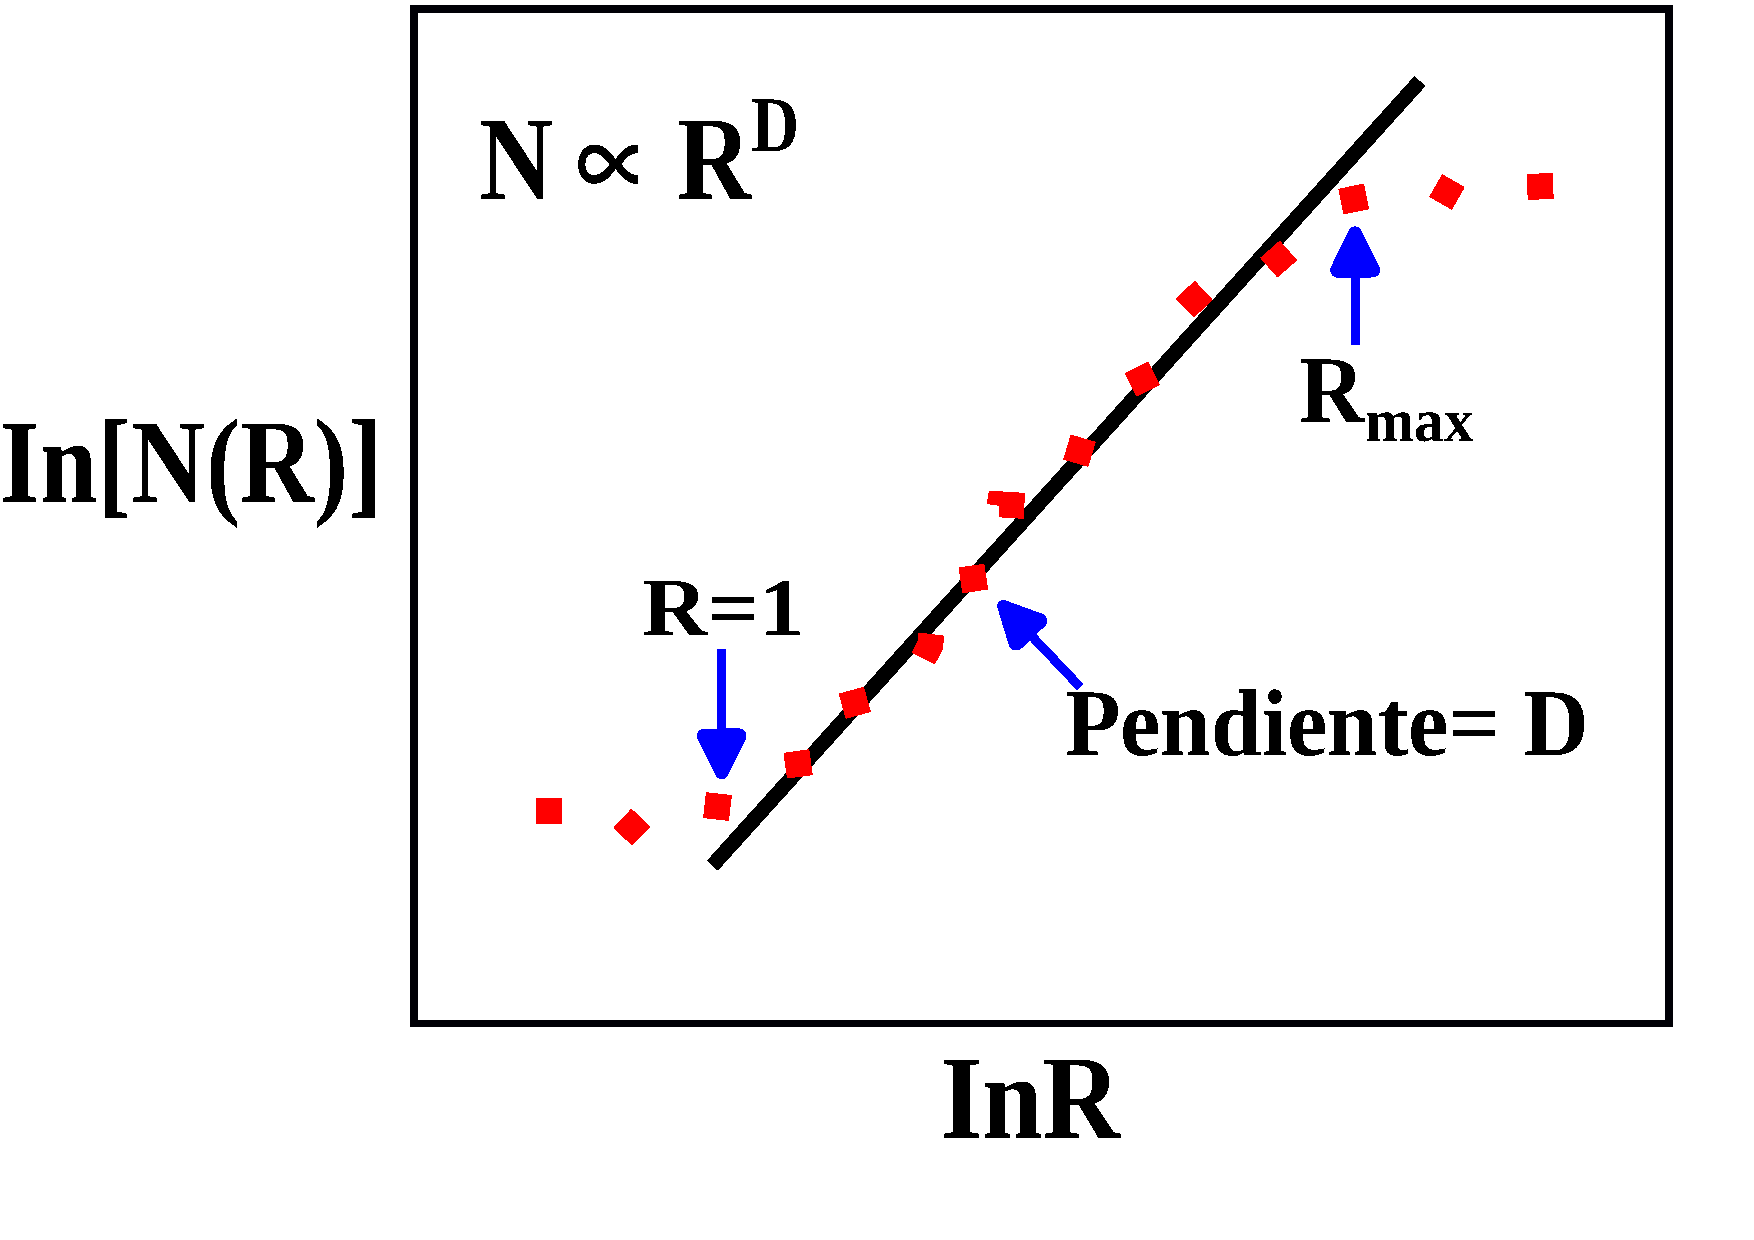
\includegraphics[width=0.5\linewidth]{graphs/dimension-fractal}
		\caption{Gr\'{a}fico de $\ln[N(R)]$ vs $\ln (R)$  del n\'{u}mero de part\'{i}culas $N(R)$ que pertenecen a un fractal que se encuentran dentro de una esfera de radio $R$. La dimensi\'{o}n fractal se obtiene ajustando una l\'{i}nea recta a los datos en la regi\'{o}n de escala.}
		\label{fig:D-Fractal}
	\end{center}
\end{figure}


\subsection*{¿Qu\'{e} es un objeto monofractal?}

Un objeto \textbf{monofractal} es un estructura fractal que puede describirse mediante una \textbf{\'{u}nica dimensi\'{o}n fractal}. Esto implica que su complejidad o irregularidad es \textbf{uniforme} en todas las escalas y regiones del objeto. Por lo tanto, su \textbf{pendiente es constante} y el mismo valor de dimensi\'{o}n fractal describe la estructura en todas las partes del objeto. Un caso concreto de monofractalidad es el estudio presentado por Enright \textit{et al.}\cite{Enright2005}, donde no se observa un cambio de pendiente (ve\'{a}se la Figura \ref{fig:Enright-Fractal}), probablemente por la pequeña cantidad de puntos que se presentan en su an\'{a}lisis y la distancia que hay entre los puntos. Adem\'{a}s, Enright \textit{et al.} calcul\'{o} la dimensi\'{o}n fractal de masa como un promedio espacial (usando esferas conc\'{e}ntricas y radio de giro), lo que posiblemente captura esta monofractalidad.

\begin{figure}[H]
	\begin{center}
		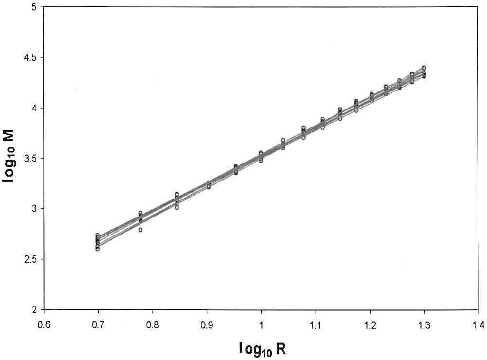
\includegraphics[width=0.4\linewidth]{graphs/Enright2005}
		\caption{Gr\'{a}fico de $\log_{10}M$ vs $\log_{10}R$ para la prote\'{i}na \textbf{Sialidase}, donde los valores de $M$ son las masas encerradas por esferas conc\'{e}ntricas de radio $R$ centradas en un \'{a}tomo. Imagen tomada de Enright \textit{et al} \cite{Enright2005}.}
		\label{fig:Enright-Fractal}
	\end{center}
\end{figure}

\section{Multifractalidad}

Otro concepto desarrollado por B. Mandelbrot en su libro \textit{Fractal Geometry of Nature} fue la multifractalidad. La multifractalidad es una propiedad de ciertos sistemas o estructuras complejas que presentan un crecimiento fractal pero de manera heterog\'{e}nea en distintas regiones o escalas. A diferencia de los fractales, que son descritos con una \'{u}nica dimensi\'{o}n fractal (un valor constante que representa la relaci\'{o}n entre el detalle del patr\'{o}n y la escala), en un sistema multifractalidad existen multiples dimensiones fractales que reflejan la variablidad de la distribuci\'{o}n y concentraci\'{o}n de sus elementos. 

En t\'{e}rminos simples, un sistema multifractal est\'{a} compuesto de distintas subestructuras que tienen diferentes grados de ``irregularidad'', lo que significa que cada regi\'{o}n del sistema podr\'{i}a necesitar una dimensi\'{o}n fractal espec\'{i}fica para describir su complejidad.

\section*{Objetos multifractales y sistemas magnetoreol\'{o}gicos}

Un objeto \textbf{multifractal} es una estructura fractal que requiere un \textbf{conjunto de dimensiones fractales} para ser descrita completamente. La complejidad del objeto \textbf{var\'{i}a localmente} y est\'{a} distribuida de manera \textbf{heterog\'{e}nea}, es decir, existen m\'{u}ltiples pendientes que dependen de la regi\'{o}n del objeto o de la medida que se est\'{e} analizando y es com\'{u}n en fen\'{o}menos naturales o en sistemas ca\'{o}ticos. Un ejemplo claro es el trabajo realizado por Carillo \textit{et al.} \cite{Carrillo2003}, donde los sistemas 
magnetorreol\'{o}gicos y otros conglomerados formados por procesos de agregaci\'{o}n, mostraron multifractalidad, que se manifiesta en la variaci\'{o}n de la dimensi\'{o}n fractal a lo largo de diferentes etapas del proceso de formaci\'{o}n 
de estructuras (v\'{e}ase la Figura \ref{fig:Carrillo-Fractal}). En t\'{e}rminos simples, en la Figura \ref{fig:Carrillo-Fractal}, se observa que en los puntos de $\log_{10}N(r)$ vs $\log_{10}r$ se pueden clasificar en tres conjuntos, cada conjunto sigue una relaci\'{o}n lineal con una pendiente definida, esto es, hay tres dimensiones fractales.


\begin{figure}[H]
	\begin{center}
		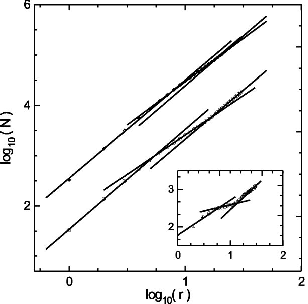
\includegraphics[width=0.4\linewidth]{graphs/Carrillo2003}
		\caption{Gr\'{a}fico de $\log_{10}N$ vs $\log_{10}r$ para estructuras formadas en un sistema magnetorreol\'{o}gico de tres etapas. La multifractalidad es una propiedad de ciertos sistemas complejos donde la estructura exhibe autosimilitud a m\'{u}ltiples  escalas. Modificado de Carrillo \textit{et al} \cite{Carrillo2003}.}
		\label{fig:Carrillo-Fractal}
	\end{center}
\end{figure}

Los sistemas magnetoreol\'{o}gicos son fluidos complejos que contienen part\'{i}culas magn\'{e}ticas (\'{o}xidos de metales) suspendidos en un l\'{i}quido (como aceite de silicona). La caracter\'{i}stica principal de estos sistemas es que sus propiedades mec\'{a}nicas cambian dr\'{a}sticamente cuando se aplica un campo magn\'{e}tico externo. En ausencia de este campo, el fluido se comporta como un l\'{i}quido ordinario, pero al aplicar un campo magn\'{e}tico, las part\'{i}culas magn\'{e}ticas se alinean y forman estructuras organizadas (como cadenas o fibras) que transforman el fluido en una especie de gel envegecido o s\'{o}lido semirr\'{i}gido en cuesti\'{o}n de milisegundos. 


\begin{comment}
	\section{Multifractalidad en sistemas magnetoreol\'{o}gicos}
	
	Para observar los diferentes patrones de agregaci\'{o}n en presencia del campo magn\'{e}tico, Carrillo \textit{et al.} \cite{Carrillo2003} utilizaron bajas concentraciones de part\'{i}culas, de menos de 0.1 en fracci\'{o}n de volumen. Observando diferentes etapas del proceso de agregaci\'{o}n. Y por lo tanto, al determinar la dimensi\'{o}n fractal de masa observaron una variaci\'{o}n de la dimensi\'{o}n fractal que son precisamente las 3 porciones en la gr\'{a}fica que est\'{a}n asociadas a 3 etapas de agregaci\'{o}n.
\end{comment}
 
 
 
\section{Niveles de organizaci\'{o}n en la estructura de las prote\'{i}nas}


Las prote\'{i}nas est\'{a}n presentes en todos los sistemas vivos, desde estructuras como la hemoglobina, el tejido cerebral y una cantidad considerable de esas prote\'{i}nas se han cristalizado para
posteriormente, caracterizarse por m\'{e}todos como RMN, R-X, ME. Y una vez hecho lo anterior, los datos son enviados y son revisados por expertos biocuradores, despu\'{e}s de
ser aprobados se ponen a disposici\'{o}n de forma gratuita bajo algún dominio como el \textit{Protein Data Bank}.

Como es bien sabido, las proteínas son polímeros lineales formados por aminoácidos. Aunque en la célula se han identificado más de 60 aminoácidos diferentes, solo 20 de ellos son incorporados de manera habitual en la síntesis de proteínas.

Cada aminoácido presenta una estructura básica compuesta por un grupo amino (\ch{-NH2}), un grupo carboxilo (\ch{-COOH}), un átomo de hidrógeno (\ch{-H}) y una cadena lateral o grupo R, todos ellos unidos a un átomo de carbono central quiral (conocido como carbono \(\alpha\)). La unión covalente entre el grupo carboxilo de un aminoácido y el grupo amino de otro, con la liberación de una molécula de agua (\ch{H2O}), da lugar al denominado enlace peptídico, el cual constituye la base estructural de las cadenas polipeptídicas. Podemos describir a las prote\'{i}nas en cuatro niveles jer\'{a}rquicos (véase la Figura \ref{fig:nivelesP}):

\begin{itemize}

\item La estructura primaria donde se encuentra la secuencia de los
amino\'{a}cidos del polip\'{e}ptido. Cuando se describe la estructura primaria de una prote\'{i}na se especifica el
orden en el que aparecen los amino\'{a}cidos desde un extremo de la mol\'{e}cula hasta el otro extremo.

\item La estructura secundaria son patrones repetitivos de una estructura local, en estos
patrones se presentan la formaci\'{o}n de puentes de hidr\'{o}geno y estas interacciones locales son las
responsables de las 2 principales conformaciones secundarias de la prote\'{i}na que son denominadas $\alpha$ h\'{e}lice y lamina $\beta$.


\item La estructura terciaria \'{e}sta basada en interacciones entre grupos laterales que tienen diferentes
propiedades: como los grupos hidr\'{o}fobos y amino\'{a}cidos polares. Como resultado de esto, la cadena
polipept\'{i}dica se pliega, se enrolla y gira en la conformaci\'{o}n nativa que ésta elija (normalmente es la conformaci\'{o}n m\'{a}s estable para una determinada secuencia de amino\'{a}cidos).


\item Por último, la estructura cuaternaria es el nivel de organizaci\'{o}n que concierna a las interacciones y el ensamblaje de las subunidades proteicas, esta categor\'{i}a incluye muchas prote\'{i}nas principalmente aquellas cuyo peso molecular supera las 50,000 unidades.

\end{itemize}

\begin{figure}[h!]
	\centering
	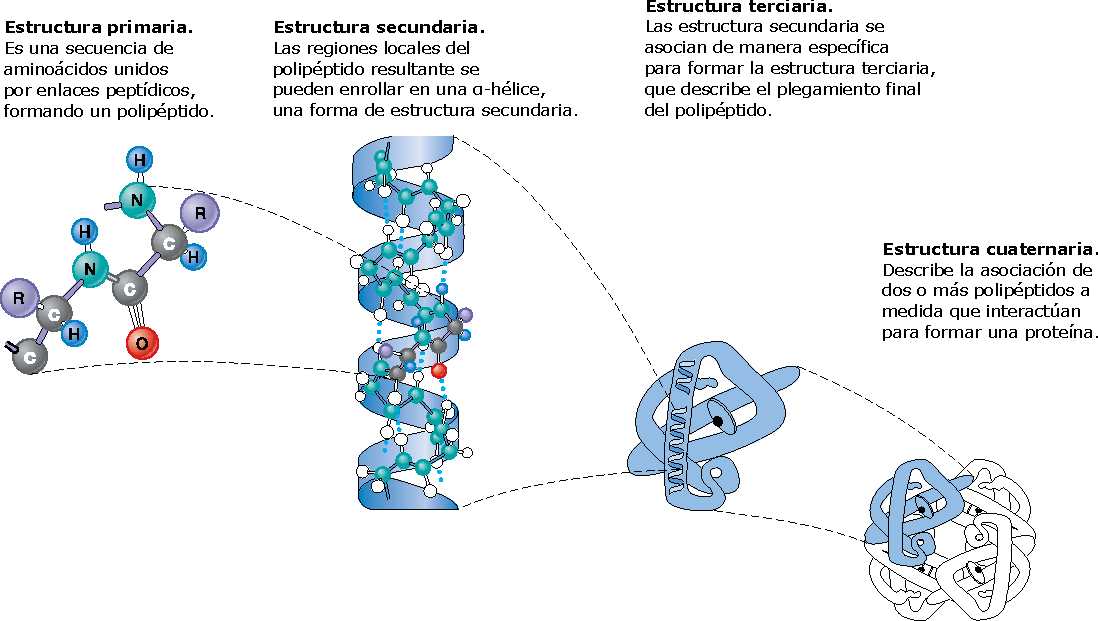
\includegraphics[width=0.9\textwidth]{graphs/niveles.pdf}
	\caption{Niveles de organizaci\'{o}n en la estructura de las prote\'{i}nas. Imagen extraida de Hardin \textit{et al.} \cite{Hardin2022}.}
	\label{fig:nivelesP}
\end{figure}

\section{Medidas para comparar estructuras proteicas}

Para evaluar y comparar estructuras proteicas a los niveles mencionados anteriormente se utilizan diferentes medidas cuantitativas y cualitativas. Aunque el problema parece sencillo su cuantificaci\'{o}n es compleja y sigue evolucionando \cite{Kufareva2012}. Una medida usada por los qu\'{i}micos computacionales es el \textit{RMSD} que significa, desviación cuadrática media de un conjunto de coordenadas atómicas (ver ecuación \ref{rmsd}). En la gr\'{a}fica que se observa en la Figura \ref{rmsd-graf} es producida mediante dinámica molecular y en ella, se estudia cómo evolucionan las posiciones de los átomos de la proteína que se analiza a través del tiempo. El \textit{RMSD} se calcula con base en una estructura de referencia que generalmente, es la posición inicial en el tiempo cero de la simulación. Es importante señalar que, esta es una medida de toda la proteína, en la gr\'{a}fica no analiza si la estructura proteica se está deshaciendo o se est\'{a} expandiendo o se está torciendo. Solo es, c\'{a}nto en promedio se desvían los \'{a}tomos de su posición original. Por lo tanto, encontrar m\'{e}todos alternativos al \textit{RMSD} o hallar enfoques complementarios para comparar estructuras sigue siendo un reto para la comunidad cient\'{i}fica.


	\begin{figure}[H]
	\hspace{-0.3cm} 
	\begin{minipage}{0.49\textwidth}
		\centering
		\begin{equation}
			RMSD = \sqrt{\frac{1}{n} \sum_{i=1}^{n} d_i^2}
			\label{rmsd}
		\end{equation}
	\end{minipage}
	\hspace{0.2cm}
	\begin{minipage}{0.49\textwidth}
		\centering
		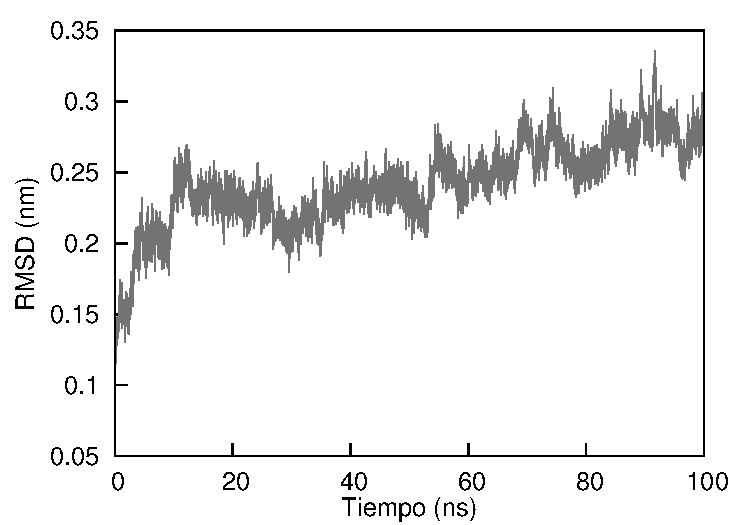
\includegraphics[width=\linewidth]{graphs/rmsd.pdf}
	\end{minipage}
	\caption{Gráfica de \textit{RMSD} a 90 ns de la proteína X.}
	\label{rmsd-graf}
	\end{figure}


\section{Metodologías para la determinación de la dimensión fractal en proteínas}

El estudio de la dimensión fractal en proteínas ha evolucionado a través de una combinación de diferentes enfoques geométricos, estadísticos y dinámicos con diferentes objetivos. La diversidad de la metodología en la literatura responde tanto a la disponibilidad de datos estructurales tridimensionales como a la interpretación física de la geometría fractal en sistemas moleculares complejos. A continuación se muestra una breve revisión al estado del arte de la dimensión fractal en sistemas proteicos.

\subsection{Primeras aproximaciones y enfoques pioneros (1980--1990)}

Las primeras tentativas de cuantificar la naturaleza fractal de las proteínas se remontan a los trabajos de Stapleton \textit{et al.}\cite{Stapleton1980} en 1980, quienes investigaron la estructura fractal de las proteínas mediante estudios de relajación de espín electrónico con hierro (Fe$^{3+}$). Los autores midieron la dependencia térmica de la tasa de relajación Raman y encontraron que la densidad de estados vibracionales sigue una ley de potencia. La dimensión fractal encontrada fue $d \approx 1.65$ que posteriormente, fue confirmada con datos de rayos X de mioglobina. Este trabajo fue pionero en demostrar experimentalmente que las proteínas tienen una estructura fractal. 

Cuatro años más tarde, Helman \textit{et al.}\cite{Helman1984} en 1984, propusieron una metodología basado en la dimensión fractal de fractones y modos vibracionales $d_{fr}$ apoyada en la teoría de Alexander-Orbach \cite{Alexander1982} sobre fractones, que depende de la topología del sistema (incluyendo los puentes de hidrógeno) y la dimensión fractal geométrica $d_f$.

Poco después, Isogai \textit{et al.} \cite{Isogai1984} desarrollaron un análisis geométrico de la estructura terciaria de 43 proteínas utilizando la teoría fractal. Su enfoque es estadístico-geométrico, sin considerar mecanismos físicos como la relajación de espín.
En su investigación lograron identifican dos regímenes fractales distintos: (1) La dimensión fractal $S$ regida por repulsiones estéricas (presentes en estructuras locales) y (2) la dimensión fractal $L$ regida por fuerzas atractivas (presentes en estructuras globales). Además, sugieren que la teoría fractal será particularmente útil para estudiar propiedades emergentes como la estabilidad conformacional, que dependen de la organización global más que de detalles locales.

Un año más tarde, Wagner \textit{et al.} \cite{Wagner1985} parte  del grupo de Stapleton \textit{et al.}, desarrollaron un método para calcular dimensiones fractales $\bar{d}$ a partir de coordenadas de carbonos $\alpha$ en 70 proteínas, estableciendo un rango de $1.27 \leq \bar{d} \leq 1.87$ y demostrando su correlación con el contenido de estructuras secundarias: $\alpha$-hélices y giros-$\beta$ aumentan $\bar{d}$, mientras que las láminas-$\beta$ lo disminuyen. Por último, descubrieron que el solvente influye en la dinámica fractal.

De manera experimental, Sow-Hsin y Teixeira \cite{Chen1986} en 1996 introdujeron un enfoque innovador para caracterizar la estructura fractal de proteínas mediante dispersión de neutrones a bajo ángulo (SANS) en complejos proteína-detergente. Observaron la formación de complejos tipo ``collar de perlas'' donde las micelas de detergente se distribuyen de forma fractal a lo largo de la cadena polipeptídica desnaturalizada. Por último, desarrollaron un modelo teórico que considera explícitamente la longitud de correlación finita, permitiendo extraer simultáneamente la dimensión fractal $D$, el tamaño micelar y el grado de desnaturalización. Encontraron que $D$ disminuye progresivamente desde 2.30 hasta 1.76 conforme aumenta la desnaturalización de la proteína.

\subsection{Consolidación de métodos geométricos y autoafines (1990--2000)}


Xin Wang \textit{et al.} \cite{Wang1990} en 1990 presentaron un método refinado para determinar las dimensiones fractales de 90 proteínas provenientes del \textit{Protein Data Bank} que abarcan cuatro clases estructurales: (1) dominios $\alpha$ antiparalelos, (2) dominios $\beta$ antiparalelos, (3) dominios $\alpha-\beta$ paralelos y (4) dominios pequeños ricos en disulfuro o ricos en metales (SD). Analizaron la relación entre la dimensión fractal y la estructura terciaria de las proteínas. El valor medio de la dimensión fractal $D_{2}$ para la estructura global de las proteínas es 1,65, muy cercano al valor teórico $\frac{5}{3}$, asociado con un \textit{random walk} en el espacio euclidiano tridimensional. Por último, encontraron que la dimensión fractal es un indicador en la evolución para proteínas homólogas y que varía de forma característica entre las clases de proteínas que analizaron proporcionando una herramienta cuantitativa para la clasificación estructural.


Cserzö y Vicsek en 1991 \cite{Cserzo1991} introdujeron un enfoque revolucionario al analizar proteínas como superficies autoafines en lugar de fractales autosimilares. Transformaron las estructuras proteicas en mapas de distancias C$\alpha$-C$\alpha$ que analizaron como superficies fractales mediante el cálculo del exponente de rugosidad $H$. Su método reveló que las proteínas nativas exhiben dos regímenes de escalado: A escalas pequeñas ($H \approx 0.32$) reflejan flexibilidad local y estructura secundaria, mientras que a escalas grandes ($H \approx 0.12$) manifiestan compactación global. Esta dualidad de escala dependiente captura esencialmente la naturaleza de las proteínas: flexibles localmente pero compactas globalmente. Desarrollaron modelos determinísticos en red cúbica que reproducen este comportamiento y demostraron que el método es suficientemente sensible para detectar diferencias entre proteínas mesófilas y termófilas, así como para monitorizar procesos de desplegamiento simulado. El trabajo de Cserzö y Vicsek representó un avance conceptual significativo al mostrar que la autoafinidad (no la autosimilitud) es el marco matemático apropiado para describir la organización estructural de las proteínas, estableciendo un puente entre la geometría local y la compactación global.


En el mismo año, Li et al. \cite{HouqiangLi1991} marca un punto de inflexión al superar la limitación de describir la superficie mediante una única dimensión fractal. Los autores introducen los conceptos \textit{fat fractal} y multifractales, argumentando que la superficie de una proteína, siendo rugosa pero de volumen finito, constituye un fractal "gordo". Asimismo, criticaron los métodos de cálculo tradicionales por su inestabilidad en sistemas autoafines y proponen el método de variación para determinar la dimensión fractal superficial $(D_G)$ de forma más fiable. Su contribución fundamental reside en demostrar la naturaleza multifractal de estas superficies a través del espectro $f(\alpha)$, revelando una heterogeneidad intrínseca donde coexisten múltiples subconjuntos fractales con distintos grados de singularidad. Esto permite explicar que regiones específicas, como el sitio activo, presentan una corrugación mayor que el promedio global, optimizando procesos como la catálisis. 

\subsection{Enfoques dinámicos y de simulación (2000--2024)}


A principios del siglo XXl Moret \textit{et al.}\cite{Moret2001} investigaron las propiedades multifractales de la hipersuperficie de energía potencial en polipéptidos y proteínas. El comportamiento multifractal se obtuvo a partir del espectro $f(\alpha)$, cuya función describe algunas propiedades estructurales de una proteína (ofreciendo una explicación alternativa a la paradoja de Levinthal). Además, encontraron que es necesario tomar en cuenta la formación de enlaces de hidrógeno ya que influye directamente en la dimensión fractal del sistema. Por otro lado, explican como el disolvente puede perturbar la estructura terciaria de una proteína y por lo tanto, modificar el comportamiento multifractal.

Cinco años más tarde, nuevamente el grupo de Moret \textit{et al.} \cite{Moret2005} investigó las propiedades fractales de 5526 cadenas proteicas diferentes a partir de un análisis de la dimensión fractal con un valor de $\delta = 2.47$, dicho grupo sostiene que este valor de dimensión proporciona una medida de la compacidad de la proteína. Indicando que el análisis multifractal puede describir algunas propiedades estructurales de las proteínas y corrobora la explicación sobre la multifractalidad en la hipersuperficie energética. Por último, sugieren que los experimentos realizados, son cruciales para determinar la mejor descripción del mecanismo de plegamiento de proteínas específicas.

Enright \textit{et al.} publicaron dos estudios que guardan una estrecha relación con el presente tema de investigación. El primero artículo publicado en 2005, Enright \textit{et al.}
\cite{Enright2005} establecieron una metodología  para calcular la dimensión fractal de masa a partir de estructuras tridimensionales obtenidas del \textit{Protein Data Bank} usando conjunto de 200 proteínas que abarcan desde 100 hasta 10, 000 aminoácidos y examinaron la variación de $D$ con el tamaño de la proteína. El valor promedio $\bar{D} = 2.5$, que es significativamente menor que un polímero tridimensional completamente compacto. También observaron que, en promedio, una proteína en su configuración nativa del \textit{Protein Data Bank} ocupa menos del $80\%$ de volumen en la proteína, lo que concuerda con una dimensión fractal de masa inferior a 3. La masa de la proteína también se ajustó al radio de giro, con un exponente de 2,5 para el conjunto de proteínas antes mencionado que corresponde estrechamente con las dimensiones fractales de masa que obtuvieron al estudiar las vibraciones de varias proteínas mediante las relaciones de Alexander-Orbach \cite{Alexander1982}.
 
 Nuevamente, Enright \textit{et al.}\cite{Enright2006} esta vez en 2006 ampliaron su estudio sobre la dimensión fractal de masa en proteínas al incorporar el efecto de la hidratación, utilizando simulaciones de dinámica molecular para analizar cómo influye el agua en la difusión vibracional. Este trabajo permitió evidenciar que la dimensión fractal varía en función del contenido de agua, y que la propagación de energía en proteínas hidratadas presenta un comportamiento anómalo, característico de sistemas con estructura fractal. Así, se estableció una conexión entre la geometría fractal de las proteínas y su dinámica energética. Como parte del estudio, se calcularon las dimensiones fractales de masa de un conjunto de 200 proteínas del \textit{Protein Data Bank}, con tamaños que oscilan entre 100 y 11,000 aminoácidos, considerando estructuras con y sin las moléculas de agua asociadas. Los resultados mostraron que la inclusión de las moléculas de agua internas y de la primera capa de hidratación produce un ligero aumento en el valor promedio de la dimensión fractal, pasando de 2.49 (sin agua) a 2.52 (con agua). Adicionalmente, se realizaron simulaciones de dinámica molecular en solución acuosa para 20 proteínas de entre 100 y 4000 aminoácidos. En este caso, al considerar explícitamente el agua de hidratación, la dimensión fractal de masa promedio se incrementó hasta 2.87, valor que se mantuvo aproximadamente constante sin depender del tamaño de la proteína. Se observó, además, que variaciones estructurales moderadas (como aquellas derivadas de un desplegamiento parcial que modifica el radio de giro en un 10\%) no afectan significativamente la dimensión fractal.


En 2024 Petreuș \textit{et al.} publicaron un estudio en que se analizó los aspectos fractales de las estructuras de las proteínas S100 para comprender mejor su complejidad. Para el cálculo de las dimensiones fractales de masa y superficie, se consideraron 33 estructuras en solución y 18 estructuras cristalinas correspondientes a las proteínas S100 humanas. El valor de la dimensión fractal de masa obtenido fue de $D_m = 1.54$, lo que confirmó la conformación extendida de los dímeros de estas proteínas según su investigación. El valor medio de la dimensión fractal de superficie es $D_s = 2,35 \cdot 0,09 $ cuando se calcula utilizando estructuras en solución y $D_s = 2,23 \cdot 0,05$ cuando se calcula utilizando estructuras cristalinas, lo que revela las irregularidades superficiales de las proteínas S100. Se han registrado cambios en las dimensiones fractales de superficie de las proteínas S100 debido a cambios en el pH del entorno, a mutaciones en sus secuencias que alteran el plegamiento de la proteína, o a sus interacciones con iones o ligandos que reflejan los reordenamientos estructurales que se producen tras la unión. Estos cambios pueden influir significativamente en la actividad biológica de la proteína, lo que convierte la dimensión fractal de la superficie en un parámetro valioso para el estudio de las funciones proteicas, sus interacciones y su posible orientación terapéutica. 

Existen otros estudios que no guardan una relación directa con el enfoque específico de esta investigación, pero abordan temáticas vinculadas al análisis proteico mediante medidas fractales. Para el lector interesado, se recomienda la consulta de las referencias \cite{Shen2001, Banerji2013, Sendker2024}. Dichos trabajos no se discuten en detalle en el presente estudio, dado que sus objetivos y, en particular, sus metodologías, se encuentran considerablemente distantes del enfoque adoptado en esta tesis.

\color{black}